\begin{figure}[t]
\centering
\subfloat[Fork-join in a loop.]{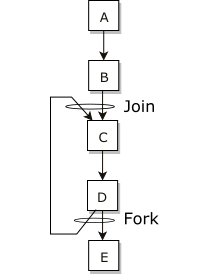
\includegraphics[width=.345\textwidth]{figures/cfg_fork_join_loop_widend}%
\label{fig:fork_join_loop}}
\hfil
\subfloat[Fork-join in an if-else statement.]{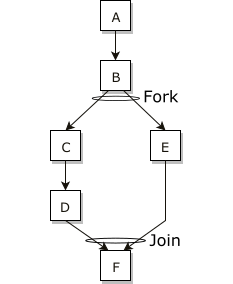
\includegraphics[width=.35\textwidth]{figures/cfg_fork_join_widend}%
\label{fig:fork_join_elif}}
\caption{Fork-join illustration in CFGs.}
\label{fig:fork_join}
\end{figure}

The fork-join model typically branches off (fork) execution at a designated point in the program, and joins (merge) at a subsequent point to resume execution. %In parallel computing, this is a technique often used to spawn multiple processes that execute in parallel, which are at some point joined to sequential execution.
%TODO: if sentence above is added, add illustration of -<==>-
When a value is defined in between the fork and join point and is forwarded to after the join it may be defined in one branch, but not or differently in the other branch or branches. When a bypass is encoded in an instruction, it is statically defined, in the sense that whatever branch is taken the value that is forwarded should always come from the bypass source that is encoded in the instruction. 


\begin{lstlisting}
$A:
   <@$\vdots$@>
$B:
   nop             || v.addi r9,  r0, 32
   nop             || v.lw   r2,  r9, 0
   nop             || v.lw   r3,  r9, 1
   addi <@\hspace{1px}\textcolor{red!70!black}{r3}\hspace{1px}@>, r0, 16 || v.lw   r4,  r9, 2
   ori  r4, r0, 0  || v.addi r10, r0, 64
$C:
   lw   r6, <@\hspace{1px}\textcolor{red!70!black}{r3}\hspace{1px}@>, 3  || v.add  r12, CP, r0
   lw   r6, <@\hspace{1px}\textcolor{red!70!black}{r3}\hspace{1px}@>, 2  || v.add  r13, CP, r0
   lw   r6, <@\hspace{1px}\textcolor{red!70!black}{r3}\hspace{1px}@>, 1  || v.add  r14, CP, r0
$D:
   nop             || v.mul  r12, r4, r12
   nop             || v.mul  r13, r3, r13
   addi r4, r4, 0  || v.add  r9,  CP, r10
   addi r4, r4, 4  || v.add  r12, r12, r13
   sfne r4, 32     || v.mul  r14, r2, r14
   bf $C           || v.add  r14, r14, r12
   addi <@\hspace{1px}\textcolor{red!70!black}{r3}\hspace{1px}@>, <@\hspace{1px}\textcolor{red!70!black}{r3}\hspace{1px}@>, 32 || v.sw   r14, r9, 0
$E:
   <@$\vdots$@>
\end{lstlisting}
%TODO: ask if i need to add loop, or change into loop.

When using the bypass network to forward a value from one basic block to another basic block, it is 

